\chapter{CryptoNight}
\section{Introduzione alle PoW ASIC-resistant}
Al fine di scoraggiare l'uso di sistemi basati su ASIC per il mining, citati nel primo capitolo, sono stati proposti diversi meccanismi PoW ASIC-resistant.
I principali algoritmi di questo tipo possono essere divisi in: PoW Multi-hash, PoW Memory-hard e PoW Programmatic.

\subsection{PoW Multi-hash}
A differenza dell'algoritmo PoW di Bitcoin che utilizza solo un tipo di funzione hash, gli algoritmi PoW Multi-hash impiegano più funzioni hash per calcolare la validità del blocco. Queste funzioni hash vengono applicate all'intestazione del blocco in una sequenza, che può essere fissa o determinata dinamicamente per ogni blocco. 
Alcuni degli algoritmi PoW multi-hash più famosi sono: \textit{X11, X14, X17, X11EVO, X16S, X16R, Quark} e \textit{TimeTravel}.

Nella ricerca scientifica di Cho, dal titolo "\textit{ASIC-Resistance of Multi-Hash Proof-of-Work Mechanisms for Blockchain Consensus Protocols}" \cite{asic1}, è stato dimostrato come gli algoritmi multi-hash non hanno una significativa differenza da altri meccanismi PoW semplici.
Inoltre, nonostante gli algoritmi di questa categoria siano spesso definiti ASIC-resistance, alcuni di loro sono già stati rotti da sistemi ASIC.
Mentre, per quanto riguarda gli algoritmi rimanenti, non è stato mai dimostrato se siano veramente resistenti agli ASIC o se semplicemente non sono ancora stati progettati ASIC specifici per essi, magari in quanto impiegati in reti piccole dal basso valore economico.

Dati i risultati ottenuti, nel paper si suggerisce di optare per l'impiego di altri meccanismi ASIC-resistant per scoraggiare effettivamente il mining basato su ASIC.

\subsection{Programmatic PoW}
Una delle nuove direzioni per meccanismi PoW resistenti è aumentare la diversità delle computazioni. 
Nell'approccio PoW Programmatic, il processo di mining coinvolge l'esecuzione di un programma che cambia frequentemente. 
Ad esempio, aggiungendo come parte della computazione un pool di funzioni matematiche o un programma generato casualmente. 

Questo rende difficile per gli ASIC ottimizzare il mining, poiché dovrebbero essere riprogrammati ogni volta che il programma cambia.
Sarebbe impraticabile costruire moduli hardware specializzati che mirino a ciascuna delle possibili attività di calcolo.  

Questo tipo di meccanismi PoW sono in fase di studio e non sono ancora stati utilizzati per la realizzazione di una vera e propria blockchain.


\subsection{PoW Memory-hard}
Infine, sebbene gli ASIC offrano una maggiore efficienza computazionale rispetto alle piattaforme di calcolo general-purpose, sono solitamente limitati in termini di memoria.
    
In un algoritmo PoW Memory-hard, il processo di mining richiede l'utilizzo di grandi quantità di memoria per importare dati complessi e calcolarne l'hash.
Una computazione in questi algoritmi richiederà il recupero di dati casuali da un grande set di dati. 
La dimensione dell'insieme sarà sufficientemente grande da rendere difficile la progettazione di un ASIC che memorizzi tutto in una memoria on-chip.

Gli algoritmi PoW memory-hard più conosciuti sono: \textit{Ethash} di Ethereum, \textit{Scrypt} e \textit{CryptNight}. 

Ad esempio, per l'algoritmo di consenso \textit{Ethash}, utilizzato nella blockchain Ethereum, 
è stato sviluppato l'ASIC Antminer E3 che ha un hash rate di 190 MH/s, che è solo 2 volte più 
veloce della GPU V100, a fronte di un consumo energetico 3 volte superiore.
Sottolineando come i processori specializzati (ASIC e FPGA) hanno un vantaggio minimo rispetto 
alle CPU e GPU a causa della complessità degli algoritmi e dell'elevato costo della memoria. 




\subsubsection{Introduzione alla Memory-Hardness di CryptoNight}
CryptoNote propone quindi CryptoNight, sul quale si entrerà in dettaglio nella prossima sezione, 
come algoritmo PoW che assicura la Memory-Hardness.
Tale proprietà è garantita grazie ad un ciclo che esegue una sequenza di letture e scritture casuali 
in una piccola area di memoria da 2MB, chiamata \textit{scratchpad}. 

L'algoritmo CryptoNight si compone di tre fasi principali:
inizializzazione dello scratchpad, il memory-hard loop ed un calcolo finale del risultato.

Nella fase 2 del loop i passaggi elencato nell'Algoritmo e nell'immagine in Figura \ref{fig:cryptonight-loop}. 
\begin{itemize}
    \item Sia A che B sono interi a 16 byte e vengono inizializzati con il risultato XOR dei byte da 0 a 31 e da 32 a 63 generati utilizzando la funzione Keccak. 
    \item Questi interi vengono quindi utilizzati come indirizzi nello scratchpad analizzando i 21 bit meno significativi. 
    Si legge il valore S[A] nello scratchpad usando A come indirizzo e si esegue la crittografia AES di S[A] con A per ottenere il risultato C. 
    \item Successivamente si esegue lo XOR su B e C e si riscrive il risultato XOR in S[A]. Si usa poi C come indirizzo, si legge S[C] in D, si moltiplicano C e D, si aggiunge il risultato della moltiplicazione ad A e si memorizza A in S[C].
    \item Infine, si ottiene il risultato XOR di A e D come nuovo A, e C come nuovo B, e si utilizeranno il nuovo A e B all'iterazione successiva. 
\end{itemize}

\begin{figure}[h!]
    \centering
    \makebox[\textwidth][c]{
    
        \begin{minipage}{0.5\linewidth}
            \centering
            \begin{algorithm}[H]
            \caption{}
            \begin{algorithmic}[1]
            \Require Integer $A$, $B$, Scratchpad memory $S$
            \Ensure Modified scratchpad memory $S$
            \For{$i \leftarrow 1$ to $524288$}
                \State $C \leftarrow \text{AES}(S[A], A)$
                \State $S[A] \leftarrow \text{XOR}(B, C)$
                \State $D \leftarrow S[C]$
                \State $A \leftarrow \text{ADD}(A, \text{MUL}(C, D))$
                \State $S[C] \leftarrow A$
                \State $A \leftarrow \text{XOR}(A, D)$
                \State $B \leftarrow C$
            \EndFor
            \end{algorithmic}
            \end{algorithm}
        \end{minipage}
        
        \hspace{0.05\linewidth}
        
        \begin{minipage}{0.45\linewidth}
            \centering
            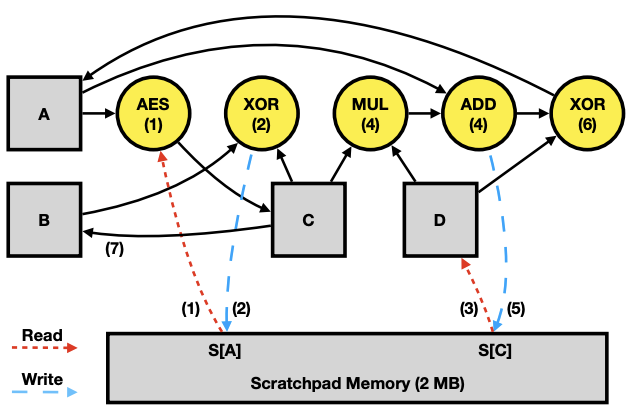
\includegraphics[width=\linewidth]{images/cryptonight.png}
        \end{minipage}
    }
    \caption{Memory-Hard loop dell'algoritmo CryptoNight. \cite{asic_memory_hard}}
    \label{fig:cryptonight-loop}
\end{figure}

Una parte del ciclo utilizza la crittografia AES per generare indirizzi di memoria casuali ai quali poi accedere.
Poiché l'output di AES è intrinsecamente casuale, non è possibile prevedere in anticipo quale sarà l'indirizzo 
di memoria successivo da leggere o scrivere. Questo impedisce la parallelizzazione del ciclo di operazioni di 
lettura e scrittura, poiché ogni iterazione dipende dal risultato dell'iterazione precedente.

Il ciclo di CryptoNight prevede 524.288 iterazioni. 
Durante ogni iterazione, viene effettuata una lettura e una scrittura casuale nello "scratchpad". 
Pertanto, l'intero ciclo comporta circa 2 milioni di operazioni di lettura e scrittura casuali. 
Questa caratteristica rende CryptoNight resistente agli attacchi con hardware specializzato come gli ASIC, 
che solitamente sfruttano la parallelizzazione per aumentare l'efficienza del mining.


\subsubsection{Risultati sperimentali}
Nel paper intitolato "\textit{Evaluating Memory-Hard Proof-of-Work Algorithms on Three Processors}" \cite{asic_memory_hard}, Feng e Luo confrontano tra loro \textit{CryptoNight}, \textit{Ethash}, \textit{Hashcash} e \textit{Cuckoo} su CPU, GPU e KNL, giungendo alla conclusione che la Memory-Hardness può essere raggiunta sfruttando la latenza o la bandwith.

I compiti che dipendono dalla latenza sono più adatti per CPU, grazie alla loro gerarchia di cache ben sviluppata. 
Al contrario, i compiti che richiedono una grande larghezza di banda possono sfruttare appieno il potenziale delle GPU.

Nel caso di studio, CryptoNight implementa una resistenza alla memoria mediante la latenza, sfruttando il tempo di accesso alla memoria per rendere più difficile la creazione di hardware specializzato.

Tuttavia, come seconda considerazione, viene specificato che, poiché i processori si stanno evolvendo rapidamente, gli algoritmi di Proof-of-Work dovrebbero essere adattabili e flessibili affinché le loro proprietà possano essere mantenute il più a lungo possibile. 



\subsection{La vittoria degli ASIC su CryptoNight}
CryptoNight rimase immune agli ASIC per un lungo periodo. Tuttavia, a partire dal 2018 vennero annunciati diversi modelli di ASIC per CryptoNight (Bitmain, Baikal e Halong Mining), capaci di raggiungere un hashrate superiore ai 200 KH/s.


\subsubsection{Bitmain}
Il 15 marzo 2018, Bitmain, un'azienda cinese, ha annunciato l'Antminer-X3, un ASIC progettato appositamente per il mining di criptovalute basate su CryptoNight. Secondo le specifiche riportate sul sito di Bitmain, l'X3 ha un tasso di hash totale di 220 kH/s e un consumo energetico di 465W.

È interessante notare la risposta su Twitter del responsabile del progetto Monero all'epoca, Riccardo Spagni, il quale sottolinea l'inefficacia dell'Antminer-X3 per la blockchain di Monero (Figura \ref{fig:Antminer-X3}).
Al tempo Monero utilizzava come PoW proprio CryptoNight, tuttavia come parte del suo protocollo blockchain adotta regolarmente hard fork pianificati e di emergenza al fine di mitigare qualsiasi potenziale minaccia derivante dagli ASIC.

% https://www.getmonero.org/2018/02/11/PoW-change-and-key-reuse.html

\begin{figure}[h!]
    \centering
    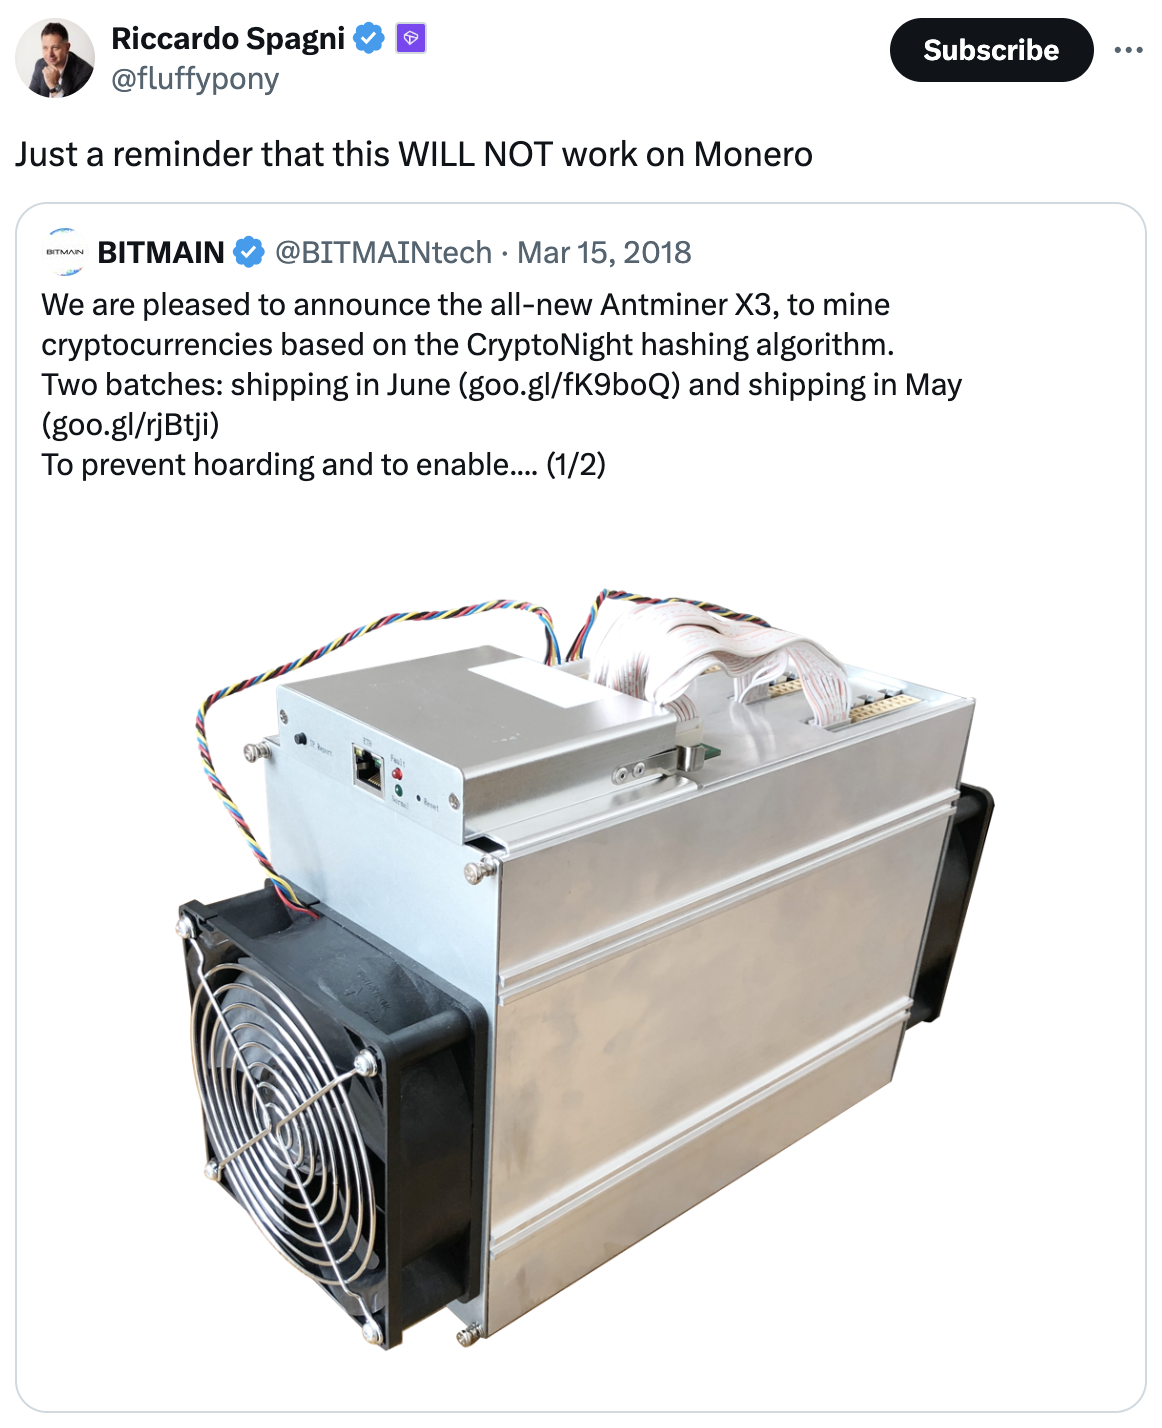
\includegraphics[width=0.45\linewidth]{images/Antminer-X3.png}
    \caption{Modello Antminer-X3 (Bitmain)}
    \label{fig:Antminer-X3}
\end{figure}

La strategia adottata da Monero gli conferisce immunità agli ASIC come l'X3 e quelli che presentati nelle prossime sezioni. 
Tuttavia, tali dispositivi rimangono utili per il mining di altre criptovalute basate su CryptoNight, come Bytecoin, Dinastycoin, Karbo e vecchie fork di Monero, che non implementano misure simili.



\subsubsection{Baikal}
Anche la società russa Baikal Mining ha reagito prontamente, rilasciando un primo modello meno potente nello stesso mese del concorrente cinese e un secondo modello più performante alcuni mesi dopo.
Entrambi gli ASIC sono in grado di minare gli algoritmi CryptoNight e CryptoNight-Lite.

\begin{itemize}
    \item[(a)] Modello BK-N, rilasciato nel marzo 2018 con un hashrate massimo di 80 kH/s ed un consumo di 120W (Figura \ref{fig:Baikal BK-N}),
    \item[(b)] Modello BK-N240, rilasciato nel maggio 2018 con un hashrate massimo di 480 kH/s ed un consumo di 650W (Figura \ref{fig:Baikal N240}).
\end{itemize}

\begin{figure}[h!]
    \centering
    \begin{subfigure}[b]{0.15\linewidth}
        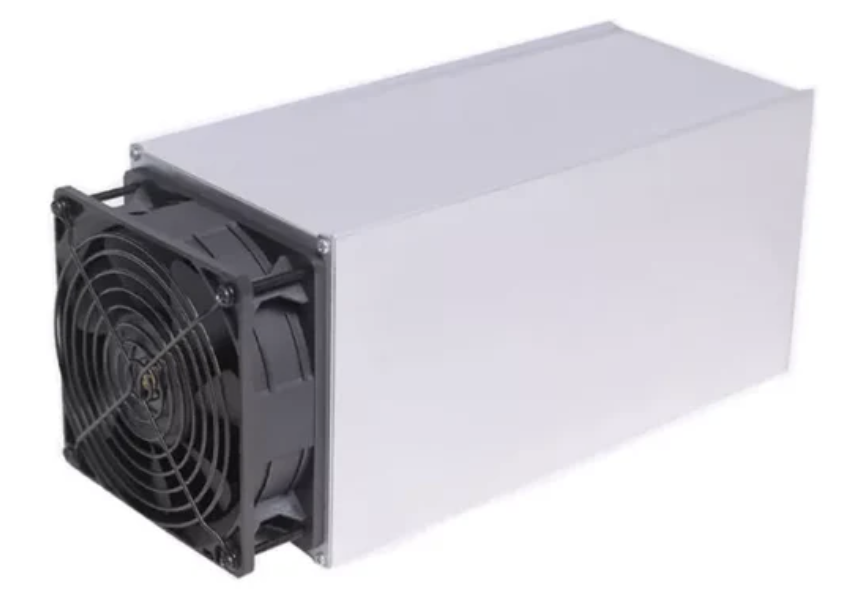
\includegraphics[width=\linewidth]{images/Baikal BK-N.png}
        \caption{}
        \label{fig:Baikal BK-N}
    \end{subfigure}
    \hspace{1.5cm}
    \begin{subfigure}[b]{0.15\linewidth}
        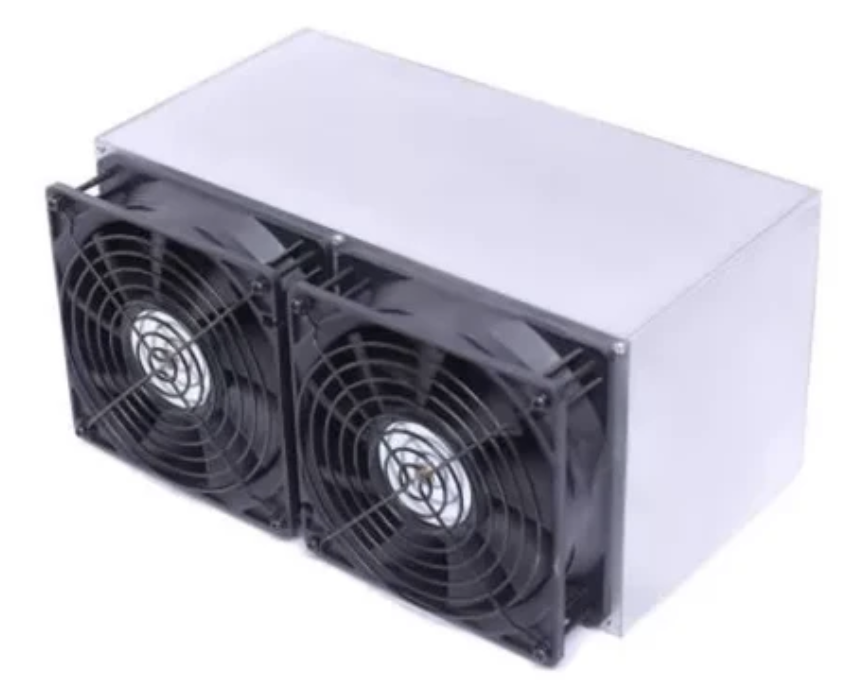
\includegraphics[width=\linewidth]{images/Baikal N240.png}
        \caption{}
        \label{fig:Baikal N240}
    \end{subfigure}
    \caption{Modelli ASICS BK-N e BK-N240 (Baikal)}
    \label{fig:Baikal miners}
\end{figure}


\subsubsection{Halong Mining}
Con un mese di ritardo, nell'Aprile 2018, anche l'azienda statunitense Halong Mining ha rilasciato il suo Modello DragonMint X2, in grado di minare l'algoritmo CryptoNight con un hashrate massimo di 248 kH/s e un consumo energetico di 490W.

\begin{figure}[h!]
    \centering
    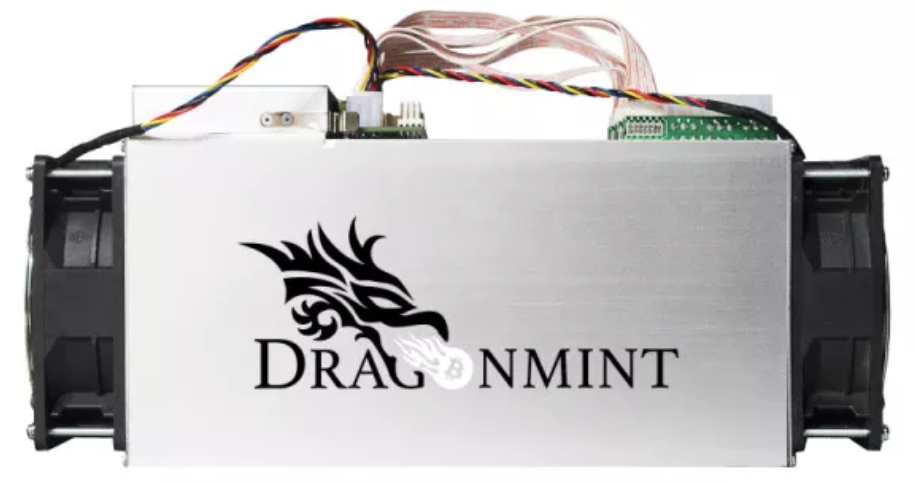
\includegraphics[width=0.2\linewidth]{images/DragonMint X2.png}
    \caption{Modello ASICS DragonMint X2 (Halong Mining)}
\end{figure}



\section{Funzione di hash CryptoNight}\label{funzione-di-hash-cryptonight}
In questa sezione si parlerà del cuore del protocollo di consenso
CryptoNote, la funzione di hash \textbf{CryptoNight}, completa con le
sue specifiche e il suo funzionamento. 

Una \textbf{funzione di hash} è una funzione che trasforma dati di
dimensione arbitraria in dati di dimensione fissata. L'operazione deve
essere simile ad una funzione casuale per garantire la distribuzione
uniforme dei risultati, indipendentemente dalla natura dei dati o
dalle precedenti iterazioni dei dati.

Come già descritto, l'obiettivo di CryptoNote era il design di una
funzione hash che fosse facilmente eseguibile da CPU consumer-grade,
disponibili nei computer normali attraverso l'esecuzione di cifrature
AES, la moliplicazione di numeri a 64 bit e l'utilizzo di uno scratchpad
che, come da specifiche dell'algoritmo, entra nella dimensione di una
classica cache L3 di un processore dell'epoca (circa 2MB). 


\subsubsection{Scratchpad}
Uno scratchpad è una grande area di memoria temporanea e non
persistente dove si possono eseguire calcoli senza alcuna conseguenza
sullo stato a lungo termine.

La dimensione dello scratchpad è definita a 2MB in quanto:

\begin{itemize}[noitemsep]
\item
  Si adatta alla cache L3 (per core) dei processori moderni, che
  diventeranno mainstream tra qualche anno;
\item
  Un megabyte di memoria interna è quasi una dimensione inaccettabile
  per il moderno pipeline ASIC;
\item
  Le GPU possono eseguire centinaia di istanze simultanee, ma sono
  limitate in altri modi: la memoria GDDR5 è più lenta della cache L3
  della CPU e notevole per la sua larghezza di banda, non per la
  velocità di accesso casuale.
\item
  Un'espansione significativa dello scratchpad
  richiederebbe un aumento delle iterazioni, il che implica a sua volta
  un aumento del tempo complessivo. Chiamate "pesanti" in una rete P2P
  senza fiducia possono portare a gravi vulnerabilità, perché i nodi
  sono obbligati a verificare il proof-of-work di ogni nuovo blocco. Se
  un nodo impiega una quantità considerevole di tempo per ogni
  valutazione dell'hash, può essere facilmente soggetto
  a attacchi DDoS da parte di una valanga di oggetti falsi con dati di
  lavoro arbitrari (valori di nonce).
\end{itemize}






\subsubsection{Primitive crittografiche utilizzate}\label{primitive-crittografiche-utilizzate}
CryptoNight è basato su delle primitive crittografiche specifiche, composte da 
\begin{itemize}
  \item
  Cifratura AES a 256bit
  \item 5 funzioni di hash, finaliste
  nella competizione per la ricerca di un nuovo standard per le funzioni
  di hash del 2012 condotto dal NIST:
  \begin{itemize}
    \item Keccak
    \item BLAKE
    \item Groest1
    \item JH
    \item Skein
  \end{itemize}
\end{itemize}

\subsection{Prima parte: Inizializzazione dello
scratchpad}\label{prima-parte-inizializzazione-dello-scratchpad}

L'input della funzione di hash (in Monero, ad esempio, di dimensione 80
bytes) viene passato nella funzione di hash di Keccak\cite{bertoni2011keccak}. Viene scelta con
\texttt{b\ =\ 1600}, quindi con dimensione dell'output di 1600 bit o 200
bytes e con dimensione del digest di 512 bits o 64 bytes con il
parametro \texttt{c\ =\ 512}. Questi byte saranno definiti come
\textbf{Keccak state} \cite{keccak_parameters}

I byte \texttt{0..31} risultanti dall'output della funzione vengono
scelti come chiave per l'algoritmo di cifratura AES-256. La chiave non
viene utilizzata così com'è, ma viene espansa\cite{standard2001federal} in 10 sotto-chiavi, con lo
scopo di rendere l'algoritmo più sicuro, utilizzando più di una chiave
AES per cifrare. L'espansione viene fatta dividendo la chiave in 8
parole di 4 byte ciascuna. Per generare le due parole rimaste al fine
completare i 10 \emph{key rounds} , si esegue la rotazione
dell'ultima parola generata, effettuata con la funzione
\texttt{RotWord()}, che esegue una permutazione ciclica e avendo come
input {[}\emph{a0,a1,a2,a3}{]} ritorna {[}\emph{a1,a2,a3,a4}{]}.
Successivamente vengono sostituiti i byte utilizzando una \textbf{S-Box}
e viene eseguito uno XOR con una costante chiamata \texttt{Rcon} (Round
constant). I dettagli di una pseudo implementazione del codice per
l'espansione della chiave è presente qui.

\begin{figure}[h!]
  \centering
  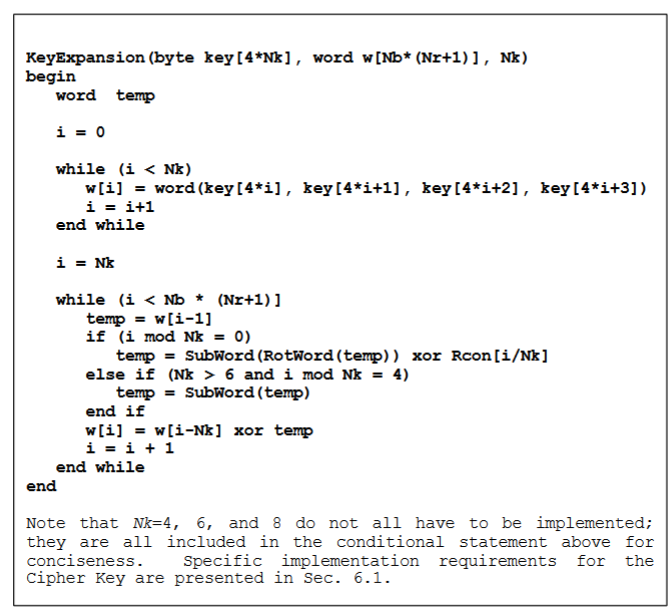
\includegraphics[width = 0.60\textwidth]{image8.png}
  \caption{Pseudoimplemetazione codice cifratura}
\end{figure}
\newpage

Viene allocato uno \textbf{scratchpad} di 2097152 bytes.\cite{crypto_note_standard_cryptonight}
Dall'output di Keccak vengono estratti i byte \texttt{64...191} e divisi
in 8 blocchi di 16 byte ciascuno. Ogni blocco viene cifrato utilizzando
il seguente codice:

\begin{algorithm}
  \caption{AES Rounds}
  \begin{algorithmic}[1]
  \For{$i = 0$ \textbf{to} $9$}
      \State block = \texttt{aes\_round}(block, round\_keys[$i$])
  \EndFor
  \end{algorithmic}
  \end{algorithm}


\subsubsection{Funzione cifratura AES}\label{funzione-cifratura-aes}

La funzione \texttt{aes\_round} esegue un round di cifratura AES, che
consiste nell'eseguire i passaggi seguenti sul blocco:

\begin{itemize}
\item
  SubBytes: ogni byte del blocco viene sostituito con un valore criptato
  utilizzando una tabella di sostituzione \emph{S-Box}.
\item
  ShiftRows: le righe del blocco vengono spostate di una posizione.
\item
  MixColumns: le colonne del blocco vengono mescolate utilizzando una
  matrice 4x4 nota come MDS, progettata per essere difficile
  da invertire.
\item
  Infine, il risultato è XORato con la chiave specifica per quel round.
  A differenza della classica funzione AES per cifrare, il primo e
  l'ultimo round quando si usano le \emph{round-keys} non sono speciali.
\end{itemize}

I blocchi che ne risultano vengono riportati nei primi 128 byte dello
scratchpad. Questi ultimi vengono cifrati nuovamente nello stesso modo,
e il risultato viene scritto nei successivi 128 byte. Questa operazione
viene effettuata 10 volte, per riempire tutto lo scratchpad di dati
pseudo-randomici. I byte \texttt{64..191}, che chiameremo
\emph{payload}, sono cifrati in questo modo 10 volte. 

\begin{figure}[h!]
  \centering
  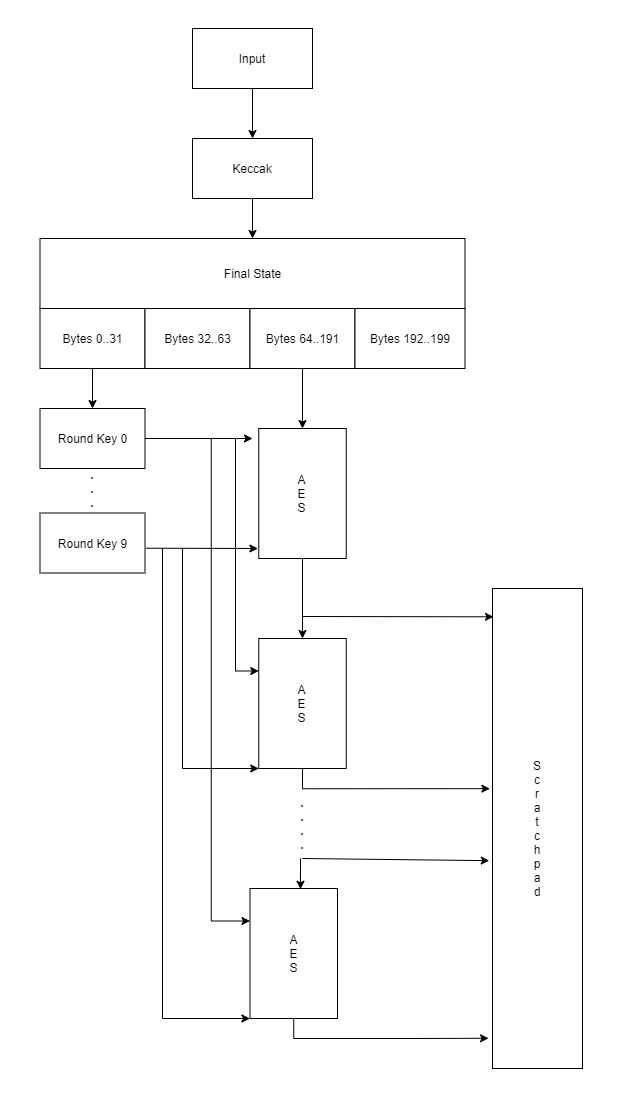
\includegraphics[width = 1\textwidth]{image_pt1.png}
  \caption{Diagramma inizializzazione scratchpad CryptoNight}
  \label{fig:my_label}
\end{figure}

\subsection{Seconda parte: Loop
memory-hard}\label{seconda-parte-loop-memory-hard}

La seconda parte si compone di un algoritmo che mantiene lo stato
composto da 52488 iterazioni. Si utilizzano operazioni
CPU-friendly, come la cifratura AES, XOR, moltiplicazioni e addizioni di
8 byte, per avere come unico

Prima di eseguire il loop utilizzato per rendere questa funzione di hash
\emph{memory-hard}, viene eseguito lo XOR sui byte \texttt{0..31} e i
byte \texttt{32..63} dell'output dell'hashing Keccak. I 32 byte
risultanti vengono utilizzati per inizializzare due variabili da 16 byte
ciascuna, \texttt{a} e \texttt{b}. Queste variabili vengono utilizzate
nel loop principale, composte da quattro passaggi:

\begin{enumerate}
\def\labelenumi{\arabic{enumi}.}
\item
  Il codice calcola l'indirizzo di memoria della variabile \texttt{a} e
  lo scrive sullo scratchpad. Per convertire un valore di 16 byte in un
  indirizzo nello scratchpad, bisogna interpretarlo come un intero
  rappresentato in little-endian, con gli ultimi 21 bit che
  rappresentano l'indice all'interno dei byte; gli ultimi 4 bit vengono
  comunque cancellati per ottenere l'allinamento a 16 byte, dato che i
  dati vengono letti e scritti sullo scratchpad in blocchi da 16 byte.
\item
  Successivamente, viene applicatata la funzione per cifrare il blocco
  \texttt{aes\_round} sull'indirizzo letto dallo scratchpad, con il
  valore di \texttt{a} usato come chiave.
\item
  Il risultato di questa operazione passa da uno XOR e il valore della
  variabile \texttt{b}, oltre ad essere scritto sullo scratchpad, sempre
  come indirizzo di memoria.
\item
  L'indirizzo ricavato viene letto dallo scratchpad e viene effettuata
  l'operazione di moltiplicazione chiamata \texttt{8byte\_mul}. Questa
  funzione, usa i primi 8 byte di ogni argomento, interpretati da essa
  come \texttt{uint\_64}, con rappresentazione little-endian. Il
  risultato di questa operazione viene convertito in 16 byte,
  concludendo l'operazione di moltiplicazione scambiando le due metà del
  risultato (8 byte ciascuna)
\item
  Il valore di \texttt{a} viene aggiunto, componente per componente in
  modulo 2\^{}64, al risultato della moltiplicazione con le due metà già
  scambiate attraverso la funzione \texttt{8byte\_add} che utilizza i
  primi 64 bit come intero senza segno, con il risultato che viene
  portato in 16 byte e scritto nello scratchpad.
\item
  Infine, viene letto l'indirizzo del risultato della cifratura
  dell'indirizzo della variabile di \texttt{a}, utilizzando come chiave
  \texttt{a} (il risultato del secondo passaggio) e viene effettuata un
  operazione di XOR con il risultato della addizione precedente.
\item
  Il risultato dell'operazione 6 viene utilizzato come nuovo valore
  della variabile \texttt{a}, mentre il risultato del passaggio 2 viene
  utilizzato come nuova variabile \texttt{b}.
\end{enumerate}



\begin{figure}[h!]
  \centering
  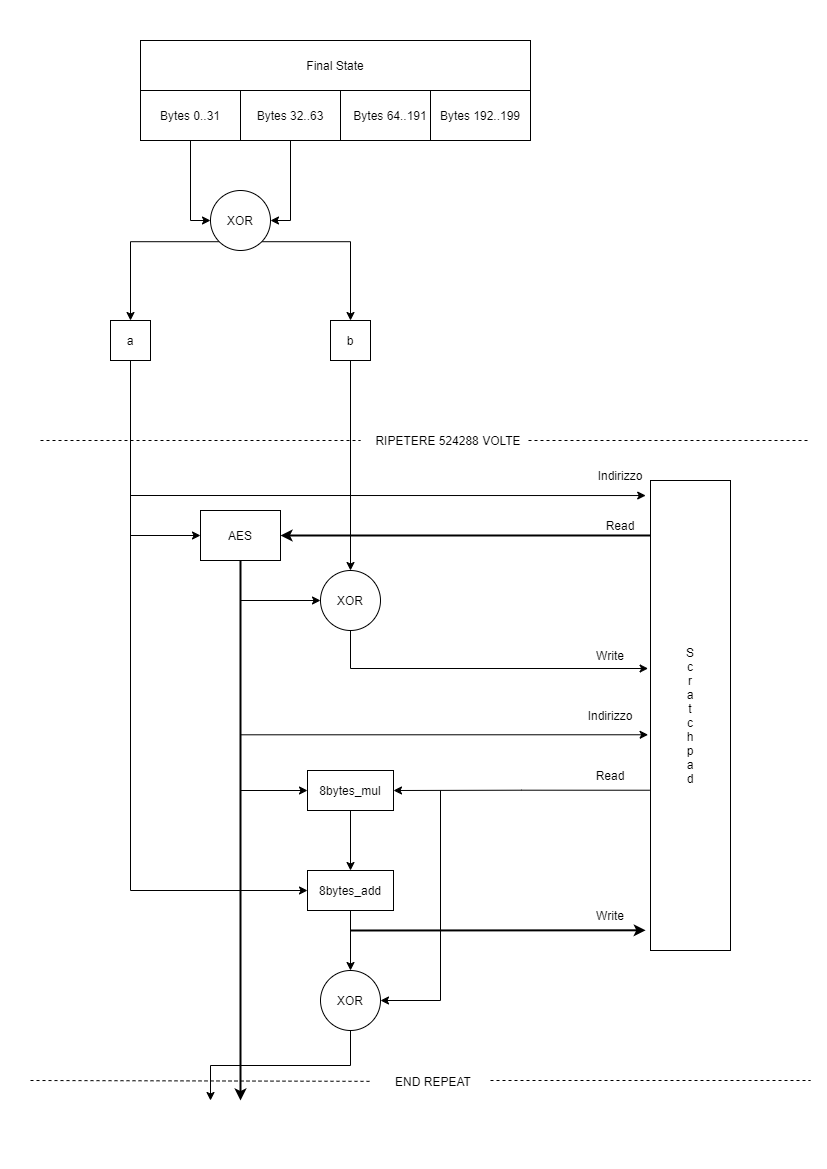
\includegraphics[width = 1\textwidth]{image_pt2.png}
  \caption{Diagramma loop memory-hard CryptoNight}
  \label{fig:my_label}
\end{figure}

\subsection{Terza parte: Calcolo del
risultato}\label{terza-parte-calcolo-del-risultato}

Dopo aver effettuato le operazioni memory-hard, i byte \texttt{32..63}
dati dall'hashing effettuato con Keccak vengono espansi in 10
\emph{round-keys} come nella prima parte.

I byte \texttt{64..191} dello stesso hashing vengono presi e viene
effettuato uno XOR con i primi 128 byte dello scratchpad. Il risultato
di questa operazione viene criptato con la funzione \texttt{aes\_round}
come nella prima parte, ma con le chiavi ricavate dall'espansione dei
byte \texttt{32..63}.\\
Il risultato di questa cifratura viene passato da uno XOR con i 128
bytes successivi dello scratchpad, cifrati nuovamente con la stessa
funzione, fino ad arrivare agli ultimi 128 byte dello scratchpad. Dopo
aver cifrato gli ultimi 128 byte viene effettuato lo XOR con gli ultimi
128 byte dello scratchpad.

I byte \texttt{64..191} del **Keccak state* vengono sostituiti con Il
risultato dell'operazione effettuata in precedenza. Tutti i 200 byte
dello stato di Keccak vengono passati da una permutazione, chiamata
\emph{Keccak-f}, con parametro \texttt{b\ =\ 1600}, l'implementazione
più sicura. Questa operazione viene effettuate per mescolare i bit dello
stato Keccak, in modo da rendere difficile la criptoanalisi del flusso
di dati.

Infine, i due bit più a destra vengono utilizzati per selezionare una
funzione di hash:

\begin{itemize}
  \item 
  0: BLAKE-256\cite{aumasson2008sha}
  \item
  1: Groest1-256\cite{groestl}
  \item 
  2: JH-256\cite{jh}
  \item 
  3: Skein-256\cite{skein}
\end{itemize}

L'output di questa funzione di hash viene applicato al Keccak state, e
l'hash risultante è l'output di CryptoNight. I diagrammi sottostanti rappresentano le operazioni
appena descritte graficamente.

\begin{figure}[h!]
  \centering
  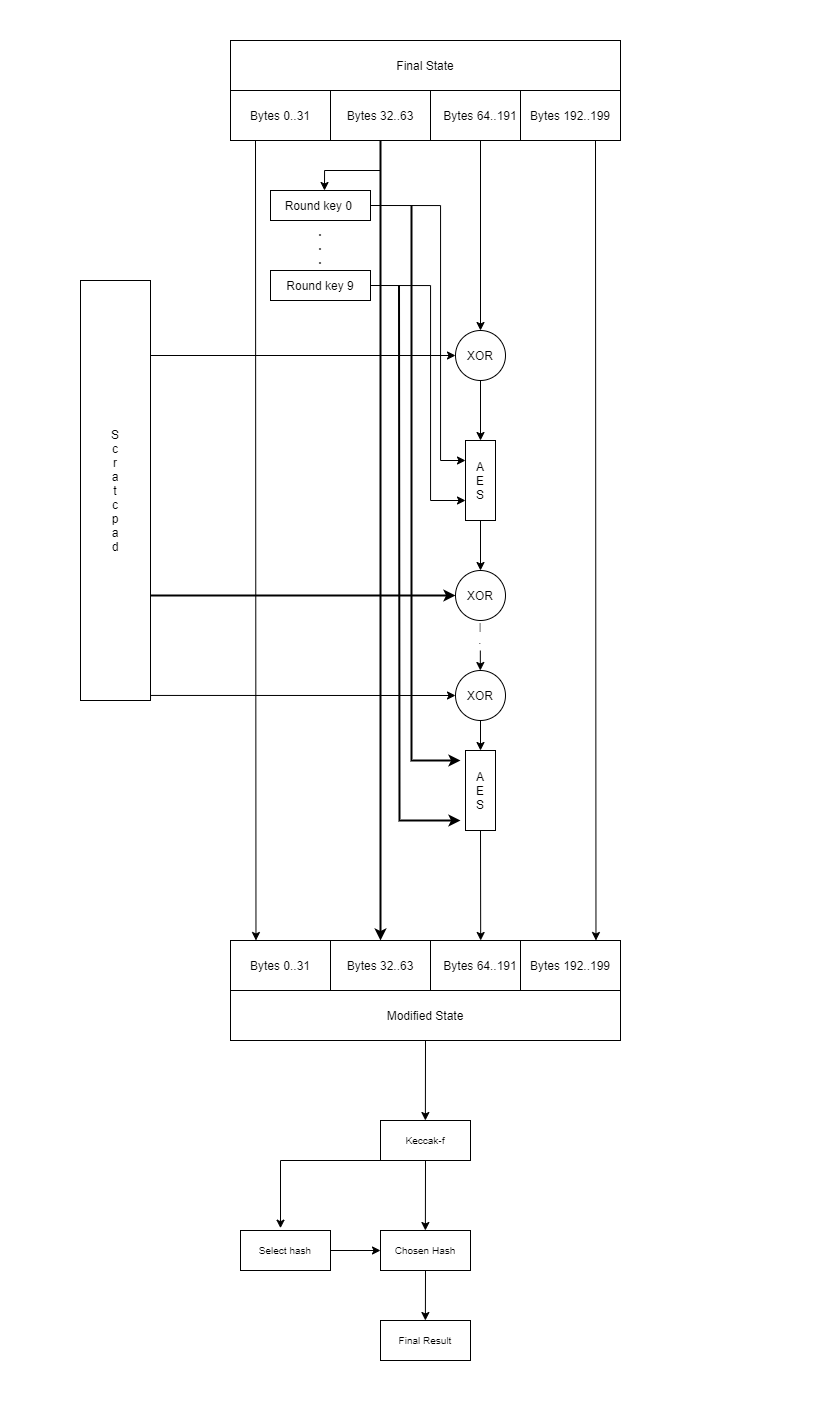
\includegraphics[width = 1\textwidth]{image_pt3.png}
  \caption{Diagramma calcolo del risultato dell'algoritmo CryptoNight}
  \label{fig:my_label}
\end{figure}